\documentclass[a4paper,oneside]{memoir}

\usepackage[left=2.5cm,right=2.5cm,top=3cm,bottom=3cm]{geometry}
\setlength{\parindent}{0.0in}
\setlength{\parskip}{0.1in}

\usepackage{graphicx}
\usepackage{xcolor}
\definecolor{red}{HTML}{AD1737}
\definecolor{chapnum}{gray}{0.6}

\usepackage{hyperref}
\hypersetup{colorlinks=true, linkcolor=blue,  anchorcolor=blue, citecolor=blue, filecolor=blue, menucolor=blue, urlcolor=blue} 

\renewcommand{\rmdefault}{pbk}
\pagestyle{plain}
\setcounter{secnumdepth}{0}

\newfont{\chapnum}{eurb10 scaled 10000}
\makechapterstyle{mike}{%
  \renewcommand{\printchaptername}{}
  \renewcommand{\chapternamenum}{}
  \renewcommand{\printchapternum}{%
    \marginpar{%
      \vspace{-20pt}
      \color{red}\chapnum \thechapter
      \vspace{20pt}
    }%
  }%
  \renewcommand{\afterchapternum}{}
  \renewcommand{\printchaptertitle}[1]{%
    \vspace{-140pt}
    %\raggedright\LARGE{##1}
  }%
}

\usepackage{wrapfig}

\newcommand{\q}[1]{``#1''}
\newcommand{\term}[1]{\textit{{#1}}}

\includeonly{%
  %partone,%
  %parttwo,%
  %partthree,%
  partfour,%
  %partfive,%
  %partsix,%
  appendix%
}
\begin{document}
\chapterstyle{mike}
  \chapter{Lesson 1}
\section{Introduction}
The web has a vast number of resources available for learning how to play
guitar. You can learn how to play songs, how to repair your broken instrument,
how to play fancy scales, and much more. The trouble is, there just aren't many
GOOD guitar lessons available to someone looking to start playing guitar. These
guitar lessons are designed for people who own (or have borrowed) a guitar, but
don't yet know the first thing about playing it.

\subsection{What you'll need for these Guitar Lessons}
%
\begin{itemize}
\item A guitar with six strings. Any type of guitar will work fine.
\item A guitar pick. Medium gauged picks are recommended to start with, but any will work okay in a pinch.
\item A chair without arms.
\item A reasonable amount of patience.
\end{itemize}
%
\subsection{Guitar Lesson Overview: What you'll learn}
By the end of this guitar lesson, you will have learned: the names of many
parts of the guitar, the names of the open strings, the process of tuning the
guitar, how to hold and use a pick, how to play a chromatic scale, and how to
play a simple song using Gmajor, Cmajor, and Dmajor chords. 

\section{Parts of a Guitar}
Although there are many different types of guitars (acoustic, electric,
classical, electric-acoustic, etc.), they all have many things in common. The
diagram to the left illustrates the various parts of a guitar.

At the top of the guitar in the illustration is the "headstock", a general term
which describes the part of the guitar attached to the slimmer neck of the
instrument. On the headstock are "tuners", which you will use to adjust the
pitch of each of the strings on the guitar.

% add the image describing the parts of a guitar
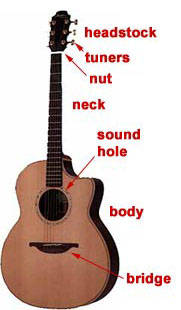
\includegraphics{partone/partsofaguitar.jpg}

At the point in which the headstock meets the neck of the guitar, you'll find
the "nut". A nut is simply a small piece of material (plastic, bone, etc.), in
which small grooves are carved out to guide the strings up to the tuners.

The neck of the guitar is the area of the instrument you'll concentrate a great
deal on: you'll put your fingers on various places on the neck, in order to
create different notes.

The neck of the guitar adjoins the "body" of the instrument. The body of the
guitar will vary greatly from guitar to guitar. Most acoustic and classical
guitars have a hollowed out body, and a "sound hole", designed to project the
sound of the guitar. Most electric guitars have a solid body, and thus will not
have a sound hole. Electric guitars will instead have "pick-ups" where the
soundhole is located. These "pick-ups" are essentially small microphones, which
allow the capture the sound of the ringing strings, allowing them to be
amplified.

The strings of the guitar run from the tuning pegs, over the nut, down the
neck, over the body, over the sound hole (or pick-ups), and are anchored at a
piece of hardware attached to the body of the guitar, called a "bridge". 

\section{The neck: A closer look}
% insert image of the neck
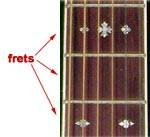
\includegraphics{partone/frets.jpg}

Examine the neck of your guitar. You'll notice there are metal strips running
across it's entire surface. These pieces of metal are referred to as "frets" on
a guitar. Now, here's what you'll need to keep in mind: the word "fret" has two
different meanings when used by guitarists. It can be used to describe:
%
\begin{enumerate}
\item The piece of metal itself
\item The space on the neck between one piece of metal and the next 
\end{enumerate}
%
To further explain, the area of the neck between the nut and the first strip of
metal is referred to as the "first fret". The area on the neck between the
first and second strip of metal is referred to as the "second fret". And so
on... 

\section{Holding a Guitar}
Now, that we know about the basic parts of a guitar, it's time to get our hands
dirty, and start learning to play it. Get yourself an armless chair, and take a
seat. You should be sitting comfortably, with your back against the back of the
chair. Slouching significantly is a no-no; you'll not only end up with a sore
back, you'll develop bad habits on the guitar.

Now, pick up your guitar, and hold it so the back of the body of the instrument
comes in contact with your stomach/chest, and the bottom of the neck runs
parallel to the floor. The thickest string on the guitar should be the closest
to your face, while the thinnest should be closest to the floor. If this isn't
the case, turn the guitar the in other direction. Typically, a right-handed
person will hold the guitar so the headstock points to the left, whereas a
left-handed person will hold the guitar so the headstock points to the right.
(NOTE: to play the guitar as a lefty would, you will need a left-handed
guitar.)

When playing the guitar sitting down, the body of the guitar will rest on one
of your legs. In most styles of guitar playing, the guitar will rest on the leg
farthest away from the headstock. This means, a person playing the guitar in a
right-handed fashion will typically rest the guitar on his/her right leg, while
someone playing the guitar in a lefty manner will rest it on their left leg.
(NOTE: proper classical guitarist technique dictates the exact OPPOSITE of the
above, but for this lesson, let's stick to our initial explanation)

Next, concentrate on your "fretting hand" (the hand closest to the neck of the
guitar, when sitting in proper position). The thumb of your fretting hand
should rest behind the neck of the guitar, with your fingers in a slightly
curled position, poised above the strings. It is extremely important to keep
these fingers curled at the knuckles, except when specifically instructed not
to do so. 

\section{Holding a Pick}
Hopefully, you've found, bought or borrowed a guitar pick. If not, you'll need
to buy yourself some. Don't be stingy, go and pick up at least 10 of them -
guitar picks are easy to lose (they often don't cost more than 30 or 40 cents
each). You can experiment with different shapes and brands, but I highly
recommend medium gauge picks to start; ones that aren't too flimsy, or too
hard.

The following documentation explains how to hold, and use a pick. When reading,
keep in mind that your "picking hand" is the hand which is nearest to the
bridge of the guitar, when sitting in the correct position.

%insert image of the pick

\includegraphics{partone/howtoholdapick.jpg}

\begin{enumerate}
\item Open your picking hand, and turn the palm to face you.
\item Close your hand to make a very loose fist. Your thumb should remain beside your index finger.
\item Rotate your hand until you are looking at it's profile, with your thumb's knuckle facing you.
\item With your other hand, slide your guitar pick between your thumb and index finger. The pick should be approximately located behind the knuckle of the thumb.
\item Be sure the pointed end of the pick is pointing directly away from your fist, and is protruding by about a half an inch. Hold the pick firmly.
\item Position your picking hand over the soundhole of your acoustic guitar, or over the body of your electric guitar. Your picking hand, with thumb knuckle still facing you, should hover over the strings.
\item Do not rest your picking hand on the strings or body of the guitar.
\item Using your wrist for motion (rather than your entire arm), strike the sixth (lowest) string of your guitar in a downward motion. If the string rattles excessively, try striking the string a bit softer, or with less of the pick surface.
\item Now, pick the sixth string in an upwards motion.
\item Repeat the process several times. Try and minimize motion in your picking hand: one short picking stroke downwards, then one short picking stroke upwards. This process is referred to as "alternate picking"
\item Try the same exercise on the fifth, fourth, third, second, and first strings.
\end{enumerate}
%
\subsection{Tips}
\begin{itemize}
\item Holding the pick in this manner will invariably feel awkward at first. You will initially have to pay special attention to your picking hand whenever you play guitar.
\item Try and create fluidity in your alternate picking. Your downstrokes should sound virtually identical to your upstrokes.
\end{itemize}

\section{Tuning}
Unfortunately, before you begin playing, you'll really need to tune your
guitar. The problem is, it is, at first, a relatively difficult task, one that
becomes much easier over time. If you know of anyone who plays guitar, who
could do the job for you, it is advised that you get them to tune your
instrument. Alternately, you could invest in a "guitar tuner", a relatively
inexpensive device which listens to the sound of each string, and advises you
(via a few blinking lights) on what you need to do in order to get the note in
tune.

If neither of these options are realistic for you, however, don't fear. You can
learn to tune your instrument, and with some patience and a bit of practice,
you'll become a pro at doing it.
\href{http://guitar.about.com/od/beginners/ss/how_tune_guitar.htm}{Learn to
tune your guitar}.

\section{Playing a Scale}
% insert a picture of a hand
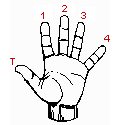
\includegraphics{partone/pickinghand.png}

Now we're getting somewhere! In order to become skillful on the guitar, we'll
need to build the muscles in our hands, and learn to stretch our fingers.
Scales are a good, albeit a not very exciting way to do this. Before we start,
look at the diagram above to understand how fingers on the "fretting hand" (the
hand that plays notes on the neck) are commonly identified. The thumb is
labelled as "T", the index finger is the "first finger", the middle finger is
the "second finger", and so on. 

\subsection{The Chromatic Scale}
%insert picture of the scale
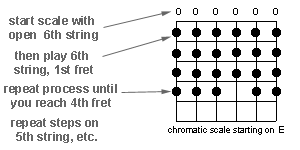
\includegraphics{partone/chromaticscale.png}

The above diagram may look confusing... fear not, it's one of the most common
methods of explaining notes on the guitar, and is actually quite easy to read.
The above represents the neck of the guitar, when looked at head on. The first
vertical line on the left of the diagram is the sixth string. The line to the
right of that is the fifth string. And so on. The horizontal lines in the
diagram represent the frets on the guitar... the space between the top
horizontal line, and the one below it is the first fret. The space between that
second horizontal line from the top and the one below it is the second fret.
And so on. The "0" above the diagram represents the open string for the string
it is positioned above. Finally, the black dots are indicators that these notes
should be played.

Start by using your pick to play the open sixth string. Next, take the first
finger on your fretting hand (remembering to curl it), and place it on the
first fret of the sixth string. Apply a significant amount of downward pressure
to the string, and strike the string with your pick.

Now, take your second finger, place it on the second fret of the guitar (you
can take your first finger off), and again strike the sixth string with the
pick.

Now, repeat the same process on the third fret, using your third finger. And
lastly, on the fourth fret, using your fourth finger. There! You've played all
the notes on the sixth string. Now, move to the fifth string... start by
playing the open string, then play frets one, two, three and four.

Repeat this process for each string, altering it only on the third string. On
this third string, play only up to the third fret. When you've played all the
way up to the first string, fourth fret, you've completed the exercise.

\subsection{Tips}
\begin{itemize}
\item When playing a note, place your finger at the "top of fret" (the area of the fret farthest away from the headstock). This will produce a clearer sound.
\item Try to use alternate picking while attempting this exercise. If this is overwhelming, try using only downstrokes with your pick, but learn properly once you've gotten used to the scale.
\item Once you've finished the scale, try playing the scale backwards, by starting at the first string, fourth fret, and playing all notes in exactly the reverse order.
\end{itemize}

\section{Playing Basic Chords}
Although practicing the previous chromatic scale will certainly provide you
with great benefits (like limbering up your fingers), it is admittedly not a
whole lot of fun. Most people love to play "chords" on the guitar. Playing a
chord involves using your pick to strike at least two notes (often more) on the
guitar simultaneously. The following are three of the most common, and easy to
play chords on the guitar. 

\subsection{Playing a G major chord}
% image of Gmajor
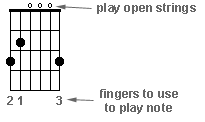
\includegraphics{partone/opengmajor.png}

This diagram illustrates the first chord we are going to play, a G major chord
(often simply called a "G chord"). Take your second finger, and put it on the
third fret of the sixth string. Next, take your first finger, and put it on the
second fret of the fifth string. Lastly, put your third finger on the third
fret of the first string. Make sure all of your fingers are curled, and are not
touching any strings they're not supposed to. Now, using your pick, strike all
six strings in one fluid motion. Notes should ring all together, not one at a
time (this could take some practice). Voila! Your first chord.

Now, check to see how you did. While still holding down the chord with your
fretting hand, play each string (starting with the sixth) one at a time,
listening to be sure each note rings out clearly. If not, study your hand to
determine why it doesn't. Are you pressing hard enough? Is one of your other
fingers touching that string, which is preventing it from sounding properly?
These are the most common reasons why a note does not sound. If you're have
trouble, read this feature on getting your chords to ring clearly. 

\subsection{Playing a C major chord}
% image of Cmajor
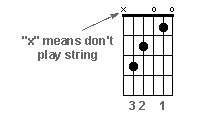
\includegraphics{partone/opencmajor.png}

The second chord we'll learn, the C major chord (often called a "C chord"), is
no more difficult than the first G major chord.

Place your third finger on the third fret of the fifth string. Now, put your
second finger on the second fret of the fourth string. Finally, put your first
finger on the first fret of the second string.

Here's where you have to be slightly careful. When playing a C major chord, you
do NOT want to strum the sixth string. Watch your pick to make sure you only
strum the bottom five strings when you are first learning the C major chord.
Test this chord as you did with the G major chord, to make sure all notes are
ringing clearly. 

\subsection{Playing a D major chord}
% image  of Dmajor
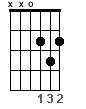
\includegraphics{partone/opendmajor.png}

Some beginners have slightly more difficulty playing a D major chord (often
called a "D chord"), since your fingers have to cram into a fairly small area.
Shouldn't be too much of a problem, however, if you can comfortably play the
other two chords.

Place your first finger on the second fret of the third string. Then, put your
third finger on the third fret of the second string. Lastly, place your second
finger on the second fret of the first string. Strum only the bottom 4 strings
when playing a D major chord.

Spend some time familiarizing yourself with these three chords... you will use
them for the rest of your guitar-playing career. Make sure you can play each of
the chords without looking at the diagrams. Know what the name of each chord
is, where each finger goes, and which strings you strum or do not strum. 

\section{Learning Songs}
We now know three chords: G major, C major, and D major. Let's see if we can
put them to use in a song. At first, switching chords will take far too long to
be able to play any songs properly. Don't give up, though! With a bit of
practice, you'll be playing away, sounding great (this tutorial on switching
chords quickly might also be of some help). In our next lesson, we'll start
learning about strumming, so you can come back to these songs, and be able to
play them better.

Here are a few of the songs you can play with G major, C major, and D major chords: 

Leaving on a Jet Plane - performed by John Denver
NOTES: when playing the G and C chord, strum them 4 times each, but when playing the D chord, strum it 8 times
MP3: iTunes download
(the strumming pattern is different in the mp3, but it should nonetheless give you an idea of how the song sounds)

The Gambler - performed by Kenny Rogers
NOTES: these aren't the exact chords for the song, but they'll do for now. Try strumming each chord one time, letting them ring.
MP3: iTunes download
(the mp3 of The Gambler is in a different key than the guitar tab, but again, it will give you an idea of how the song sounds) 

Brown Eyed Girl - performed by Van Morrison
NOTES: There is one chord in this song that we don't know yet, but it's only used briefly. Skip it for now. Try strumming each chord four times.
MP3: iTunes download

\section{Practice Schedule}
Realistically, to start improving on guitar, you're going to need to set aside
a bit of time to practice. Developing a daily routine is a good idea...
planning to spend at least 15 minutes daily practicing all you've learned will
really help. At first, your fingers will be sore, but by playing daily, they'll
toughen up, and in a short amount of time, they'll stop hurting. The following
list should give you an idea of how to spend your practice time:
%
\begin{itemize}
\item Get your guitar in tune.
\item Make sure you're sitting, holding the guitar, and using your pick properly. You'll have to correct your natural bad habits at first, until it becomes second nature.
\item Play the chromatic scale several times. Try playing it backwards.
\item Play each of the three chords you've learned. Check to be sure each note is ringing. If not, find out why, and correct the problem.
\item Try moving from one chord to another. Before switching chords, mentally picture exactly where each finger is going to move in order to play the next chord. Only then should you switch chords. This is the key to switching chords quickly. 
\item If you're having trouble getting your chords to ring clearly, read this feature on getting your chords to ring clearly.
\item Try playing some, or all of the songs listed above. At first, try only to think of the songs as a way in which to practice playing chords.
\item Don't get discouraged. This is hard stuff at first, and you'll probably feel like you can't do it. You certainly can. Everyone struggles, so just put in your 15 minutes, and then don't worry about it until the next time you play. This is supposed to be fun! 
\end{itemize}
%
That's it for now! Once you're comfortable with this lesson, move on to lesson
two, which includes information on the names of the guitar strings, plus more
chords, more songs, and even several basic strumming patterns. Good luck, and
have fun! 


  \chapter{Lesson 2}
\section{Introduction}
In lesson one of this special feature on learning the guitar, we were
introduced to the parts of the guitar, learned to tune the instrument, learned
a chromatic scale, and learned Gmajor, Cmajor, and Dmajor chords. If you are
not familiar with any of these, be sure to read lesson one before proceeding.

\subsection{What You'll Learn in Lesson Two}

This second lesson will continue to focus on exercises to strengthen the
fingers in the fretting hand. You'll also learn several new chords, in order to
play many more songs. String names will also be discussed in this feature.
Lastly, lesson two will also introduce you to the basics of strumming the
guitar.

Are you ready? Good, let's start lesson two.

\section{A New Scale}
% insert the scale image
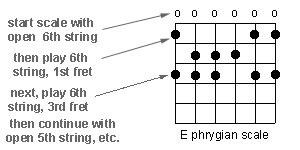
\includegraphics{parttwo/ephrygianscale.png}

To play this scale, we need to review which fingers to use to play which notes
on the fretboard. In the following scale, we will use our first finger to play
the all notes on the first fret of the guitar. Our second finger will play all
notes on the second fret. Our third finger will play all notes on the third
fret. And, our fourth finger will play all notes on the fourth fret (since
there aren't any in this scale, we won't use our fourth finger at all). It is
important to stick to these fingerings for this scale, because it is an
efficient way of using our fingers, and is a concept we will continue to use in
upcoming lessons.

\subsection{E phrygian (fridge-ee-n)}

One of the best ways to start working on the co-ordination in your fingers is
to practice playing scales. Although they may seem boring, they will certainly
help build the strength and agility your fingers need to play the guitar well.
Keep that in mind while practicing this new scale.

Start by using your pick to play the open sixth string. Next, take the first
finger on your fretting hand, and place it on the first fret of the sixth
string. Play that note. Now, take your third finger, place it on the third fret
of the sixth string, and play the note. Now, it's time to move on to playing
the open fifth string. Keep following the diagram, playing each note indicated
until you have reached the third fret on the first string.

\subsection{Remember:}
%
\begin{itemize}
\item To use alternate picking throughout. Try starting the scale with a
      downstroke, then next time try starting the scale with an upstroke.
\item Once you've finished the scale, try playing the scale backwards, by
      starting at the first string, third fret, and playing all notes in exactly the
      reverse order.
\item The key here is accuracy, not speed! Try playing the scale very slowly,
      making sure that each note is ringing clearly.
\end{itemize}

\section{Names of Guitar Strings}
%insert image of guitar strings
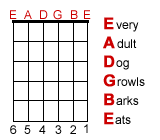
\includegraphics{parttwo/openstrings.png}

Just a little bit more technical talk before we get into playing more chords
and songs. Don't worry, this shouldn't take you more than a couple of minutes
to memorize!

Every note on the guitar has a name, represented by a letter. The names of each
of these notes is important; guitarists need to know where to find these notes
on their instrument, in order to read music.

The image to the left illustrates the names of the six open strings on the guitar.

The strings, from sixth to first (thickest to thinnest) are named E, A, D, G, B
and E again.

In order to help you memorize this, try using the accompanying phrase "Every
Adult Dog Growls, Barks, Eats" to keep the order straight.

Try saying the string names out loud, one by one, as you play that string.
Then, test yourself by pointing to a random string on your guitar, then trying
to name that string as quickly as possible. In following lessons, we'll be
learning the names of the notes on various frets on the guitar, but for now,
we'll just stick with the open strings.

\section{Learning an E Minor Chord}
% insert image of Eminor chord
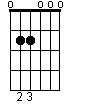
\includegraphics{parttwo/openeminor.png}

Last week, we learned three types of chords: Gmajor, Cmajor, and Dmajor. In
this second lesson, we'll explore a new type of chord\ldots{} a "minor" chord. The
terms "major" and "minor" are terms used to describe the sound of the chord. In
very basic terms, a major chord sounds happy, while a minor chord sounds sad
(listen to the difference between major and minor chords). Most songs will
contain a combination of both major and minor chords.

\subsection{Playing an E minor chord}

Easiest chord first\ldots{} playing an Eminor chord only involves using two fingers
in your fretting hand. Start by placing your second finger on the second fret
of the fifth string. Now, place your third finger on the second fret of the
fourth string. Strum all six strings, and, there you have it, an Eminor chord!

Now, like last lesson, test yourself to make sure you're playing the chord
properly. Starting on the sixth string, strike each string one at a time,
making sure each note in the chord is ringing clearly. If not, study your
fingers, and identify what the problem is. Then, try to adjust your fingering
so the problem goes away.

\section{Learning an A Minor Chord}
% insert image of Aminor chord
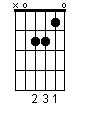
\includegraphics{parttwo/openaminor.png}

Here is another chord that gets used all the time in music, the Aminor chord.
Playing this shape shouldn't be too hard: start by placing your second finger
on the second fret of the fourth string. Now, place your third finger on the
second fret of the third string. Lastly, place your first finger on the first
fret of the second string. Strum the bottom five strings (being careful to
avoid the sixth), and you'll be playing an Aminor chord.

As with all previous chords, be sure to check each string to make sure all the
notes in the chord are ringing clearly.

\section{Learning a D Minor Chord}
% insert image of Dminor chord
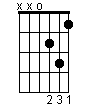
\includegraphics{parttwo/opendminor.png}

Last week, we learned how to play a Dmajor chord. In lesson two, we'll examine
how to play a Dminor chord. For an inexplicable reason, newer guitarists have a
hard time remembering how to play this chord, perhaps because it doesn't get
used as often as some others. For this reason, you should make an extra effort
to memorize a Dminor chord.

Start by placing your first finger on the first fret of the first string. Now,
put your second finger on the second fret of the third string. Lastly, add your
third finger to the third fret of the second string. Now, strum only the bottom
four strings.

Check to see if your chord is ringing clearly. Watch the Dminor chord\ldots{} be
sure you are only strumming the bottom four strings\ldots{} otherwise, the chord
might not sound so nice!

\section{Learning to Strum}
% insert image of strumming
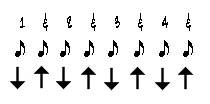
\includegraphics{parttwo/strum1.jpg}

A guitarist with a good grasp of strumming can bring a two-chord song to life.
In this first lesson on strumming, we'll examine some of the basics of
strumming the guitar, and learn a widely used strumming pattern.

Grab your guitar, and, using your fretting hand, form a G major chord (review
how to play a Gmajor chord).

The pattern above is one bar long, and contains 8 strums. It might look
confusing, so for now pay attention to the arrows at the bottom. An arrow
pointing down indicates a downward strum. Similarly, an upwards arrow indicates
that you should strum upwards. Notice that the pattern starts with a
downstroke, and ends with an upstroke. So, if you were to play the pattern
twice in a row, your hand wouldn't have to vary from it's continual down-up
motion.

Play the pattern, taking special care to keep keep the time between strums the
same. After you play the example, repeat it without any pause. Count out loud:
1 and 2 and 3 and 4 and 1 and 2 and (etc.) Notice that on the "and" (referred
to as the "offbeat") you are always strumming upward. If you are having
problems keeping a steady rhythm, try playing along with an mp3 of the
strumming pattern.

\subsection{Make Sure:}
\begin{itemize}
\item if playing an acoustic guitar, you strum over the sound hole
\item all strings ring clearly
\item Make sure the volume of your downstrums and upstrums are equal
\item Be careful not to strum too hard, as this produces an undesirable sound
\item Be careful not to strum too softly, as this will produce a "wimpy" sound.
      Your pick should be striking the strings with a relatively firm, even stroke
\item Think of your elbow as being the top of a pendulum - your arm should
      swing up and down from it in a steady motion, never pausing at any time.
\item Most of the picking motion should come from a rotation of the wrist,
      rather than from the forearm. Be sure not to keep your wrist stiff when
      playing.
\end{itemize}
%
By removing only one strum from the previous pattern, we'll create one of the
most widely used strumming patterns in pop, country, and rock music.

When we remove the strum from this pattern, the initial instinct will be to to
stop the strumming motion in your picking hand. This is exactly what we DON'T
want, as this alters the on-beat downstrum / off-beat upstrum pattern we've
established.

The key to this playing this strum successfully is to keep the strumming motion
going while slightly lifting the hand away from the body of the guitar
momentarily, on the downstroke of the third beat, so the pick misses the
strings. Then, on the next upstroke (the "and" of the third beat), bring the
hand closer to the guitar, so the pick hits the strings. To summarize: the
upward/downward motion of the picking hand should not change from the first
pattern. Deliberately avoiding the strings with the pick on the third beat of
the pattern is the only change.

Listen to, and play along with, this second strumming pattern, to get a better
idea on how this new pattern should sound. Once you are comfortable with this,
try it at a somewhat faster speed. It is important to be able to play this
accurately - don't be satisfied with getting MOST of the up and down strums in
the right order. If it's not perfect, it will make learning any harder strums
virtually impossible. Be sure that you can play the pattern many times in a
row, without having to stop because of an incorrect strum.

This is a tricky concept, and it can be guaranteed that you will have some
problems with it at first. The idea is, if you introduce basic strumming
patterns early, within a couple of lessons, you'll have gotten the hang of it,
and will be sounding great! It is important to try not to get frustrated\ldots{}
soon, this will become second nature.

\section{Learning Songs}
The addition of three new minor chords to this week's lesson gives us a total
of six chords to learn songs with. These six chords will provide you with the
opportunity to play literally hundreds of country, blues, rock, and pop songs.

If you need to refresh your memory on which chords we've learned so far, you
can review the major chords from lesson one, and the minor chords from lesson
two. Here are a few of the songs you can play with G major, C major, D major, E
minor, and A minor chords:

\nameref{sec:song4} --- performed by The Eagles

\emph{Notes} You know all of these chords, but this song will take you a while
to play well. For now, use a basic strum (only slow downstrums), and switch
chords when you reach the word that the new chord is above.

\nameref{sec:song5} --- written by Bob Dylan

\emph{Notes} this tune will also take a while to master, but if you keep at it,
you'll make progress quickly. For strumming, either strum four slow strums per
chord, or, for a challenge, use the hard strumming pattern that we learned in
this lesson.

About a Girl --- performed by Nirvana

\emph{Notes} Again, we won't be able to play the entire song, but the main
part we can do rather easily, as it only contains an Eminor and Gmajor chord.
Play the song as follows: Eminor (strum: down, down up) Gmajor (strum: down up
down up) and repeat.

\nameref{sec:song3} --- performed by Van Morrison

\emph{Notes} We learned this song last lesson, but try it again, now that you
know how to play the Eminor chord we didn't know before.

\section{Practice Schedule}
Practicing at least 15 minutes per day on the guitar is recommended. Playing
every day, even for this small amount of time, will get you comfortable with
the instrument, and you'll be amazed at your progress. Here's a schedule to
follow.
%
\begin{itemize}
\item Make sure your guitar is in tune (how to tune)
\item Go over material from lesson one. Concentrate on the chromatic scale and
      major chords.
\item Review the open string names.
\item Play the E phrygian scale several times. Play the scale forwards and
      backwards, slowly, in an even tempo. Concentrate on accuracy!
\item Spend at least five minutes on strumming. Try these patterns with
      different chords. Try playing the strumming patterns with one chord, switching
      chords, and playing the pattern again.
\item Play this week's minor chords. Say the name of the chord as you play it,
      to help with memorization. Practice switching from one minor chord to another,
      or from a minor to a major chord.
\item Try playing some, or all of the songs listed. Review songs from lesson
      one.They will certainly not sound very good at first. Try only to think of the
      songs as a way in which to practice playing chords.
\end{itemize}
%
You can see that we are quickly building a large amount of material to
practice. If you find it impossible to practice the above in one sitting, try
playing them over several days. Be sure not to ignore any of the items on the
list, even if they're not a ton of fun to practice.

You will undoubtedly sound pretty rough when you first start playing this new
material. Everyone does\ldots{} that is why we practice. If you can't seem to get
something right even after a lot of practice, shrug your shoulders, and leave
it for tomorrow.

We're done lesson two! When you're ready, move on to lesson three, we'll
discuss even more about chords, more strumming patterns, the basics of reading
music, plus new songs and more. Hope you're having fun!


  \chapter{Lesson 3}
\section{Overview}
This third lesson will include both review material, and new material. We'll learn the three remaining open chords that are generally considered the basic chords. We'll also learn another strumming pattern, and an A Blues Scale. And, as with the previous lessons, we'll finish up by learning a few new songs that use these new techniques we've learned.

Are you ready? Good, let's begin lesson three.

\section{The Blues Scale}
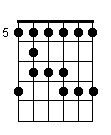
\includegraphics{partthree/bluesscale.png}

Before we jump into playing this useful new scale, let's review the fingers we will use to play the scale's notes. This scale is referred to as a "movable scale", meaning that we can play the scale anywhere on the neck. For now, we will play the scale starting on the fifth fret, but feel free to play it at the tenth fret, at the first fret, or anywhere else.

As with previous exercises, the blues scale requires precise fingering in your fretting hand in order for it to be most useful. All notes on the fifth fret will be played by the first finger. Notes on the sixth fret will be played by the second finger. Notes on the seventh fret will be played by the third finger. And all notes on the eighth fret will be played by the fourth finger.

One of the best ways to start working on the coordination in your fingers is to practice playing scales. Although they may seem boring, they will help build the strength and agility your fingers need to play the guitar well. Keep that in mind while practicing this new scale.

Count up to the fifth fret of your guitar. On most guitars, the fifth fret will be marked with a dot on the fretboard. Place your first finger on the fifth fret of the sixth string and play that note. Next, put your fourth (pinky) finger on the eighth fret of the sixth string, and again play that note. Now, continue to the fifth string, and follow the pattern illustrated above, until you've reached the eighth fret on the first string (listen to scale. Take your time and learn this scale well... it'll be one that you use often.

\subsection{Remember:}
\begin{itemize}
\item Use alternate picking.
\item Once you've finished the scale, try playing the scale backwards. Start at the first string, third fret, and play all notes in exactly the reverse order.
\item The key here is accuracy, not speed! Try playing the scale very slowly, making sure that each note is ringing clearly.
\end{itemize}

\section{Learning an E Major Chord}
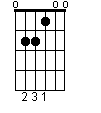
\includegraphics{partthree/openemajor.png}

Just a few more chords this week to fill in the ones we didn't cover previously. Once you've learned these three new chords, you'll know all of what are generally considered to be the basic open chords.

\subsection{Playing an E major chord}

Playing an Emajor chord is actually very similar to playing an Aminor chord; you just need to switch the strings you are playing the chord on. Start by placing your second finger on the second fret of the fifth string. Now, place your third finger on the second fret of the fourth string. Lastly, place your first finger on the first fret of the third string. Strum all six strings and you're playing an Emajor chord.

Now, like last lesson, test yourself to make sure you're playing the chord properly. Starting on the sixth string, strike each string one at a time, making sure each note in the chord is ringing clearly. If not, study your fingers, and identify what the problem is. Then, try to adjust your fingering so the problem goes away.

\section{Learning an A Major Chord}
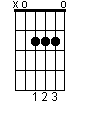
\includegraphics{partthree/openamajor.png}

This chord is a little tougher; you've got to fit all three of your fingers on the second fret, and it can feel a little crowded at first. Start by placing your first finger on the second fret of the fourth string. Next, put your second finger on the second fret on the third string. Lastly, place your third finger on the second fret of the second string. Strum the bottom five strings (being careful to avoid the sixth), and you'll be playing an Amajor chord.

Another common way to play an Amajor chord is by flattening one finger across the second fret of all three strings. This can be tricky, and initially, will be extremely difficult to play cleanly.

\section{Playing an F Major Chord}
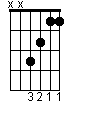
\includegraphics{partthree/openfmajor.png}

This chord has been left until last, because, honestly, it's a toughie. As the saying goes... "it's not called an F-chord for nothing!"

Many new guitarists have such a problem with the Fmajor chord because it involves a new concept; using your first finger to press down frets on two strings.

Start by placing your first finger on the first frets of both the first and second strings. Now, slightly roll the finger back (towards the headstock of the guitar). Many people find this technique makes playing the Fmajor chord slightly easier. Next, place your second finger on the second fret of the third string. Lastly, place your third finger on the third fret of the fourth string. Strum only the bottom four strings, and you're playing an Fmajor chord.

Chances are, at first, very few, if any of the notes will ring when trying to strum this chord. Check to make sure your second and third fingers are curled, and not flattened against the other strings of the guitar. Although this chord seems nearly impossible at first, within weeks, you'll have it sounding as good as the rest of the chords you play.

\section{Chord Review}
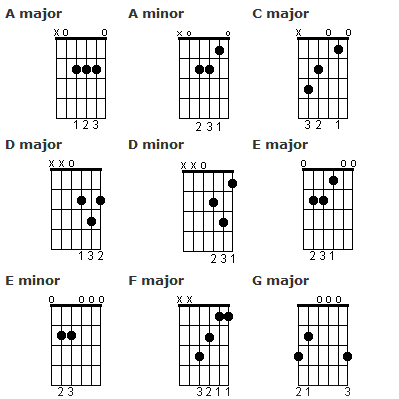
\includegraphics{partthree/lesson-three-chord-chart.png}

Including the three new chords in this week's lesson, we've now learned a total of nine chords. That might not seem like a whole lot, but at first, they can be hard to memorize. If you're having a hard time remembering all these chords, refer to the following archive.

\subsection{Practicing these chords}

Getting these chords memorized is just the first step. In order for them to be useful, you'll have to learn to move from chord to chord fairly quickly. This will take much practice and patience, but you'll get the hang of it!

Once you've reviewed these chords thoroughly, move on to learning a new strum. The main reason most beginners have trouble switching chords quickly is because of wasted movement in their fretting hand. Study your fingers when moving from chord to chord. Chances are, one (or a few) of your fingers will come way off the fretboard, and often hover in mid-air while you try to decide where each finger should go. This is unnecessary, and can really slow you down. Now, try again... play a chord, and BEFORE you switch to another chord, visualize playing this second chord shape. Picture in your mind exactly which fingers will need to go where, and only after you've done this should you switch chords. Pay attention to any small, unnecessary movements your fingers make, and eliminate them. Although this is easier said than done, your hard work and attention to detail will start paying off quickly.

\section{New Strumming Pattern}
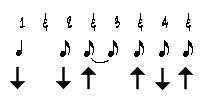
\includegraphics{partthree/strum3.jpg}

In lesson two, we learned all about the basics of strumming. If you still aren't comfortable with the concept and execution of basic guitar strumming, I suggest you return to that lesson and review.

This strum isn't much different from the one in lesson two. In fact, many guitarists find it slightly easier.

Before you try and play this pattern, take some time to learn what it sounds like. Listen to an mp3 clip of the strumming pattern, and try to tap along with it. Once you are comfortable with it, try it at a faster speed. Now pick up your guitar and try playing the pattern while holding down a Gmajor chord (be sure to use the exact upstrokes and downstrokes the diagram illustrates). If you're having trouble, put down the guitar and practice saying or tapping out the rhythm again, making sure to repeat it multiple times. If you don't have the correct rhythm in your head, you'll never be able to play it on guitar.

Remember to keep the up and down strumming motion in your picking hand constant - even when you're not actually strumming the chord. Try saying out loud "down, down up, up down up" (or "1, 2 and, and 4 and") as you're playing the pattern.

\subsection{Remember:}
\begin{itemize}
\item Make sure all strings are ringing clearly
\item Make sure the volume of your downstrums and upstrums are equal
\item Be careful not to strum too hard, as this can cause strings to rattle and produces an undesirable sound
\item Be careful not to strum too softly, as this will produce a "wimpy" sound. Your pick should be striking the strings with a firm, even stroke
\item Think of your elbow as being the top of a pendulum; your arm should swing up and down from it in a steady motion, never pausing at any time.
\item Having said that, the bulk of the picking motion should come from a rotation of the wrist, rather than from the forearm. Be sure not to keep your wrist stiff when playing.
\end{itemize}

\section{Learning Songs}
The addition of three new minor chords to this week's lesson gives us a total of nine chords to learn songs with. These nine chords will provide you with the opportunity to play literally hundreds of country, blues, rock, and pop songs. Give these songs a try:

House of the Rising Sun - performed by The Animals
NOTES: This song is a little tough at first; it uses five of the nine chords we've learned. Ignore the picking pattern for now - instead strum each chord six times quickly with only downstrums.
MP3: Amazon.com download

Last Kiss - performed by Pearl Jam
NOTES: this song is quite easy to play... it only uses four chords which repeat for the entire song. Use this week's strumming pattern for the song (play the pattern once for each chord).
MP3: Amazon.com download

Mr. Jones - performed by The Counting Crows
NOTES: This one might be tough, because it uses an Fmaj chord, and because some chords are held longer than others. Playing along with a recording of the song should help. Although this week's strumming pattern isn't exactly what they play, it will work fine.
MP3: Amazon.com download

American Pie - performed by Don McLean
NOTES: This one will be hard to memorize! It's very long, and has lots of chords, but it should be a good project. Ignore the 7ths... play Amin instead of Am7, Emin instead of Em7, and Dmaj instead of D7. Also, ignore the chords in the brackets for now.
MP3: Amazon.com download

\section{Practice Schedule}
I hope you're putting in your fifteen minutes of practice per day! It's not a lot of time to play guitar, but even fifteen minutes will yield good results over time. If you have the time to play more, it's highly encouraged... the more the better! Here's a suggested use of your practice time for the next few weeks.
\begin{itemize}
\item Make sure your guitar is in tune (review how to tune).
\item Warm up by playing the blues scale, forwards and backwards, several times. Play slowly, use alternate picking, and make sure each note rings clearly.
\item Play the E phrygian scale from lesson 2 several times, paying careful attention to detail.
\item Review all nine major and minor chords we've learned. Practice moving from chord to chord quickly.
\item Spend some time working on this week's new strumming pattern. Also, be sure to revisit the lesson two strumming patterns. Try switching from chord to chord while using these patterns.
\item Try to play one, or a few of the songs above. See if you can memorize part of a song, and the lyrics to the song. At this point, songs probably won't sound great when you try and play them, but with some patience, you'll be sounding like a pro within months! 
\end{itemize}
As was suggested in lesson two, if you find it impossible to find the time to practice all of the above in one sitting, try breaking up the material, and practicing it over several days. There is a strong human tendency to only practice things which we are already quite good at. You'll need to overcome this, and force yourself to practice the things you are weakest at doing.


  \chapter{Lesson 4}
\section{Overview}
In lesson one of this special feature on learning the guitar, we were
introduced to the parts of the guitar, learned to tune the instrument, learned
a chromatic scale, and learned Gmajor, Cmajor, and Dmajor chords. Guitar lesson
two taught us to play Eminor, Aminor, and Dminor chords, an E phrygian scale, a
few basic strumming patterns, and the names of the open strings. In guitar
lesson three, we learned how to play a blues scale, Emajor, Amajor, and Fmajor
chords, and a new strumming pattern. If you are not familiar with any of these
concepts, it is advised that you revisit these lessons before proceeding.

\subsection{What You'll Learn in Guitar Lesson Four}

We'll start adventuring a little farther up the neck in this lesson. You'll
learn a new type of chord\ldots{} what is known as a "power chord". You'll also
learn the names of the notes on the sixth and fifth string. Plus, of course,
strumming patterns, and a bunch more songs to play. Let's start guitar lesson
four.

\section{The Musical Alphabet on Guitar}

\includegraphics{partfour/musalph.jpg}

So far, most of what we've learned on the guitar has been focused on the bottom
few frets of the instrument. Most guitars have at least 19 frets - by only
using the first three, we aren't using the instrument as effectively as we
could. Learning the notes all over the guitar fretboard is the first step we
need to take to unlock the instrument's full potential

\subsection{The Musical Alphabet}

Before we begin, it is very important to understand the way the "musical
alphabet" works. It is similar in many respects to the traditional alphabet, in
that it uses standard letters (remember your ABCs?). In the musical alphabet,
however, the letters only progress up to G, after which they begin again at A.
As you continue up the musical alphabet, the pitches of the notes get higher
(when you go past G up to A again, the notes continue to get higher, they don't
start at a low pitch again.)

Another complication of learning the musical alphabet on guitar is that there
are extra frets in between some, but not all of these note names. The graphic
above is an illustration of the musical alphabet. The ties between the notes B
and C, and also between the notes E and F, reflect the fact there is NO "blank"
fret between these two sets of notes. Between ALL OTHER notes, there is one
fret space.

This rule applies to all instruments, including piano. If you are familiar with
the piano keyboard, you will know that there is no black key between the notes
B and C, and also E and F. But, between all other sets of notes, there is a
black key.

\emph{Summary} On the guitar, there are no frets between the notes B\&C, and between
E\&F. Between all other notes, there is one (for now, unnamed) fret between
each.

\section{Notes on the Neck}
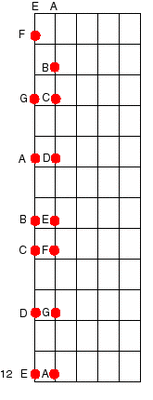
\includegraphics{partfour/fretboard.png}

From guitar lesson two, you'll remember that the name of the open sixth string
is "E". Now, let's figure out the other note names on the sixth string.

Coming after E in the musical alphabet is\ldots{} you guessed it\ldots{} F. Referencing
the musical alphabet we just learned, we know there is no blank fret between
these two notes. So, F is on the sixth string, first fret. Next, let's figure
out where the note G is located. We know that there is a blank fret between F
and G. So, count up two frets, and G is on the third fret of the sixth string.
After G, in the musical alphabet, comes the note A again. Since there is a
blank fret between G and A, we know that A is on the fifth fret of the sixth
string. Continue this process all the way up the sixth string. You can check
the diagram here to make sure you are correct.

Remember: there is also no blank fret between the notes B and C.

Once you reach the 12th fret (which is often marked on the neck of the guitar
by double dots), you'll notice you have reached the note E again. You'll find
on all six strings that the note on the 12th fret is the same as the open
string.

Once you've finished counting up the E string, you'll want to try the same
exercise on the A string. This shouldn't be difficult\ldots{} the process is exactly
the same as it was on the sixth string. All you need to know is the name of the
open string to get started.

Unfortunately, understanding how to figure out note names on the fretboard
isn't enough. For these note names to be useful, you'll have to go about
memorizing them. The best way to memorize the fretboard is to commit several
note names and frets to memory on each string. If you know where A is on the
sixth string, for example, it will be much easier to find the note B. For now,
we'll just worry about memorizing the notes the sixth and fifth strings.

In lesson five, we will fill in the blank frets in the diagram with note names.
These names include sharps (?) and flats (?). Before you start learning these
other notes, however, you'll need to understand and memorize the above notes.

\subsection{THINGS TO REMEMBER:}
\begin{itemize}
\item The musical alphabet goes from A to G, then back to A again.
\item There is no blank fret between the notes B\&C, and E\&F.
\item The note name on the 12th fret of any string is always the same as the
      open string.
\item Memorize the open string name, and several more note names and locations
      on both the sixth and fifth string. This will make finding all other notes much
      quicker.
\end{itemize}

\section{Power Chords}
In order to learn power chords effectively, you'll need to really understand
the names of the notes on the neck of the guitar. If you glossed over that
page, you'll want to revisit it, and learn it well.

\subsection{What a Power Chord Is}

In some styles of music, particularly in rock and roll, it's not always
necessary to play a big, full sounding chord. Often, especially on an electric
guitar, it sounds best to play two-or-three note chords. This is when power
chords come in handy.

Power chords have been popular since the birth of blues music, but when grunge
music started to rise in popularity, many bands chose to use power chords
almost exclusively, instead of more "traditional" chords. The power chords we
are about to learn are "movable chords", meaning that, unlike the chords we've
learned so far, we can move their position up or down the neck, to create
different power chords.

Although the power chord pictured here contains three notes, the chord contains
only two *different notes* - one note is doubled an octave higher. A power
chord contains the "root note" - the root of a C power chord is "C" - and
another note called the "fifth". For this reason, power chords are often
referred to as "fifth chords" (written C5 or E5, etc).

The power chord does not contain the note which traditionally tells us whether
a chord is major or minor. Thus, a power chord is neither major nor minor. It
can be used in a situation where either a major or a minor chord is called for,
however. Take a look at this example of a chord progression:

Cmajor - Aminor - Dminor - Gmajor

We could play the above progression with power chords, and we'd play it as follows:

C5 - A5 - D5 - G5

\subsection{Power chords on the sixth string}
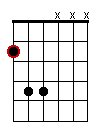
\includegraphics{partfour/powerchord6.png}

Take a look at the diagram above - note that you do NOT play the third, second,
and first strings. This is important - if any of these strings ring, the chord
won't sound very good. You'll also notice that the note on the sixth string is
circled in red. This is to denote that the note on the sixth string is the root
of the chord. This means that, while playing the power chord, whatever note is
being held down on the sixth string is the name of the power chord.

For example, if the power chord were being played starting on the fifth fret of
the sixth string, it would be referred to as an "A power chord", since the note
on the fifth fret of the sixth string is A. If the chord were played on the
eighth fret, it would be a "C power chord". This is why it is important to know
the names of the notes on the sixth string of the guitar.

Play the chord by placing your first finger on the sixth string of the guitar.
Your third (ring) finger should be placed on the fifth string, two frets up
from your first finger. Lastly, your fourth (pinky) finger goes on the fourth
string, on the same fret as your third finger. Strum the three notes with your
pick, making sure that all three notes ring clearly, and that all are of equal
volume.

\subsection{Power chords on the fifth string}
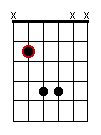
\includegraphics{partfour/powerchord5.png}

If you can play the power chord on the sixth string, this one should be no
trouble at all. The shape is exactly the same, only this time, you'll need to
be sure you don't play the sixth string. Many guitarists will overcome this
problem by lightly touching the tip of their first finger against the sixth
string, deadening it so it doesn't ring.

The root of this chord is on the fifth string, so you'll need to know what the
notes are on this string in order to know what power chord you're playing. If,
for example, you're playing a fifth string power chord on the fifth fret, you
are playing a D power chord.

\subsection{Things to Know About Power Chords:}
\begin{itemize}
\item Power chords are often referred to as a "fifth" or "5" chord. If you see
      a chord written as C5, it is a C power chord
\item You can optionally omit the pinky finger, and play a power chord as a
      two-note chord. Most guitarists stick with the 3-note version, as they sound
      more full
\item A common fingering for a power chord is to play the root note with the
      first finger, while the third finger barres the other two notes
\item Power chords are generally used in pop, rock, and blues music. Because
      they are not big, full sounding chords, power chords are not commonly used in
      acoustic strumming situations
\item Many guitarists prefer to use all downstrokes when strumming power
      chords. This results in a more "chunky" sound. This is not a rule, only an
      observation
\end{itemize}

\section{F Major Chord Review}
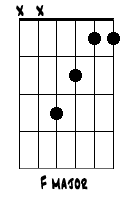
\includegraphics{partfour/chord_fmajor_open.png}

It might seem silly to devote an entire page to going over one chord we've
already learned, but, believe me, you will appreciate it in coming weeks. The F
major chord is the most difficult we've learned thus far, but it uses a
technique that we will use constantly in future lessons. That technique is
using one finger in your fretting hand to hold down more than one note at a
time.

\subsection{The F major shape}

In case you're having trouble remembering how to play the chord, let's go over
it again. Your third finger plays the third fret on the fourth string. Your
second finger plays the second fret on the third string. And, your first finger
plays the first fret on both the second and first strings. Make sure when you
strum the chord that you're not playing the sixth and fifth strings.

Many guitarists find that slightly rolling the first finger back (towards the
headstock of the guitar) makes playing the chord slightly easier. If, after
you've done this, the chord still doesn't sound properly, play each string, one
by one, and identify what the problem string(s) are. Keep practicing this chord
- play it every day, and don't give up. It won't take long for the Fmajor chord
to start sounding just as good as the rest of your chords do.

\subsection{Songs that use an F major chord}

There are, of course, thousands of songs that use an F major chord, but for
practicing purposes, here are just a few. They may take some work to master,
but you should have them sounding good with some solid practice. If have
forgotten some of the other chords we've learned, you can check the guitar
chord library.

Mother - performed by Pink Floyd
This is a good acoustic song to start with, because there aren't many chords,
the changes are slow, and F major only occurs a couple of times.

Kiss Me - performed by Sixpence None the Richer
The strum for this song is tricky (we'll leave it alone for a while\ldots{} for now,
play quick downstrums 8x per chord, only 4x for the chorus). There are a few
chords we might not have covered yet, but they should be explained at the
bottom of the page. Not many F major chords\ldots{} just enough to keep you
challenged.

Night Moves - performed by Bob Seger
Just a quick F major in this song, so it might be a difficult tune to play at
first. If you know the song well, this one will be much easier to play. 

\section{Strumming Patterns}
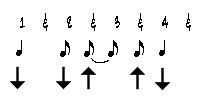
\includegraphics{partfour/strum4.png}

In lesson two, we learned all about the basics of strumming the guitar. We
added another new strum to our repertoire in lesson three. If you still aren't
comfortable with the concept and execution of basic guitar strumming, it is
advised that you return to those lessons and review.

Just a slight variation from the strum we learned in lesson three gives us
another very common, usable strumming pattern. In fact, many guitarists
actually find this pattern to be slightly easier, as there is a slight pause at
the end of the bar, which can be used to switch chords.

Before you try and play the strumming pattern above, take some time to learn
what it sounds like. Listen to an mp3 clip of the strumming pattern, to and try
to tap along with it. Repeat this until you can tap out this pattern without
thinking about it.

Once you've learned the basic rhythm of this strum, pick up your guitar and try
playing the pattern while holding down a Gmajor chord. Be sure to use the exact
upstrokes and downstrokes the diagram illustrates - this will make your life
much easier. If you're having trouble, put down the guitar and practice saying
or tapping out the rhythm again. If you don't have the correct rhythm in your
head, you'll never be able to play it on guitar. Once you're comfortable with
the strum, try playing along with the same pattern at a faster tempo (listen to
faster tempo strum here).

Again, remember to keep the up and down strumming motion in your picking hand
constant - even when you're not actually strumming the chord. Try saying out
loud "down, down up, up down" (or "1, 2 and, and 4") as you're playing the
pattern.

\subsection{Things to Remember}
\begin{itemize}
\item If playing an acoustic guitar, make sure to strum directly over the sound hole
\item On electric guitar, strum over the body, not over the neck
\item Make sure all strings are ringing clearly
\item Make sure the volume of your downstrums and upstrums are equal
\item Don't strum too hard, as this causes strings to rattle, and produces an
      undesirable sound
\item Don't strum too softly, as this produces a "wimpy" sound. Your pick
      should be striking the strings with a relatively firm, even stroke
\item Think of your elbow as being the top of a pendulum; your arm should swing
      up and down from it in a steady motion, never pausing at any time.
\item Having said that, the bulk of the picking motion should come from a
      rotation of the wrist, rather than from the forearm. Be sure not to keep your
      wrist stiff when playing.
\end{itemize}

\section{Learning Songs}
Since we've now covered all the basic open chords, plus power chords, we have a
lot of options in which songs we can play. This week's songs will be focus on
both open and power chords.

\nameref{sec:song10} (Nirvana)

This is perhaps the most famous of all grunge songs. It uses all power chords, so once you can play those comfortably, the song shouldn't be too hard.

\nameref{sec:song11} (CCR)

We can use our new strum with this fairly simple song. Although it does have a couple of chords we haven't covered yet, they should be explained well on the page.

\section{Practice Schedule}
As we progress further in these lessons, it becomes more and more important to
have daily practice time, as we're starting to cover some really tricky
material. Power chords can take a while to get used to, so I suggest making a
habit of playing them regularly. Here's a suggested use of your practice time
for the next few weeks.
%
\begin{itemize}
\item Make sure your guitar is in tune (review how to tune).
\item Warm up by playing the chromatic scale, forwards and backwards, several
      times. Play slowly, use alternate picking, and make sure each note rings
      clearly.
\item Play the E phrygian scale from lesson two several times, paying careful
      attention to detail.
\item Review the names of notes on the sixth and fifth string. Practice calling
      out a random note (e.g. C), and trying to find that note on BOTH the sixth and
      fifth string. Memorize at least two other notes, and their positions on each
      string.
\item Work on your power chords. Make sure your ring finger is positioned well
      on the appropriate fret (it is the finger that most often makes power chords
      sound bad). Slide from chord to chord, and try moving from the 6th string power
      chords to the 5th string power chords.
\item Review all nine major and minor chords we've learned. You should really
      be close to memorizing all of these chords by now. Pick two chords, and
      practice moving from one to the next quickly and smoothly. Then, pick two new
      chords, and repeat the process.
\item Spend some time working on this week's new strumming pattern. Also, be
      sure to revisit the patterns from lesson two and lesson three. Try switching
      from chord to chord while using these patterns.
\item Work on playing that pesky F major chord. Don't give up until it sounds
      perfect. Try playing some of the songs listed on that page.
\item Try to play all of the songs in lesson four. Each of these songs has been
      chosen to help you work on a particular aspect of your guitar playing.
\end{itemize}
%
We are starting to build up a large archive of things to practice, so if you
find it impossible to find the time to practice all of the above in one
sitting, try breaking up the material, and practicing it over several days.
There is a strong human tendency to only practice things which we are already
quite good at. You'll need to overcome this, and force yourself to practice the
things you are weakest at doing.

I can't emphasize strongly enough that it is important to practice everything
we've done in these four lessons. Some things will undoubtedly be more fun than
others, but trust me, the things you hate doing today are probably techniques
that will become the basis for other things you will love to play in the
future. The key to practice is, of course, fun. The more you enjoy playing
guitar, the more you'll play, and the better you will get. Try to have fun with
whatever you're playing.

In lesson five, we'll learn a blues shuffle, names of sharps and flats, a barre
chord, plus more songs! Hang in there, and have fun!


  \chapter{Lesson 5}
\section{Overview}
In lesson one of this special feature on learning the guitar, we were introduced to the parts of the guitar, learned to tune the instrument, learned a chromatic scale, and learned Gmajor, Cmajor, and Dmajor chords. Guitar lesson two taught us to play Eminor, Aminor, and Dminor chords, an E phrygian scale, a few basic strumming patterns, and the names of the open strings. In guitar lesson three, we learned how to play a blues scale, Emajor, Amajor, and Fmajor chords, and a new strumming pattern. Lesson four introduced us to power chords, basic note names on the sixth and fifth string, and new strumming patterns. If you are not familiar with any of these concepts, it is advised that you revisit these lessons before proceeding. 

\subsection{What You'll Learn in Lesson Five}

Get ready for a real challenge this week... lesson five will introduce a whole new type of chord that you'll use a lot in the future, the "barre chord". We'll also complete our learning of the note names on the sixth and fifth string, learn a blues shuffle and several guitar leads, as well as learn a bunch of new songs.

Are you ready? Good, let's start guitar lesson five. 

\section{Sharps and Flats}
In guitar lesson four, we learned the names of the notes on the sixth and fifth string (you'll want to review them first if you're unsure of them). While that lesson was designed to teach you the basic note names, it did not tell you all you need to know as a guitarist. The following lesson will fill in the gaps lesson four intentionally avoided.

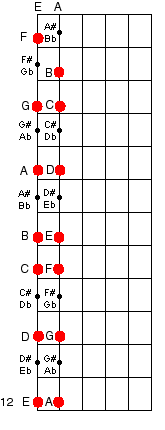
\includegraphics{partfive/fretboard_full.png}
If you've absorbed the material in lesson four, you'll know the names of all the notes in red on the diagram to the left. What you won't recognize is the names of the notes in between these red dots.

Let's begin by examining two new terms... "sharp" - which is written like this: \# , and "flat" - which is written like this: b . Essentially, the term sharp means a note is raised a note by one fret (a "semitone"), while flat means a note is lowered by one fret (a "semitone").

Upon studying the diagram to the left, you'll notice each "in-between" note has two alternate names: one being a letter name followed by a sharp sign, and the other being a letter name followed by a flat sign. To explain this, we'll name the note on the second fret of the sixth string. The note is one fret above the note F on the first fret, so we will refer to the note as an F sharp(F\#). Alternately, the same note is also one fret below the note G on the third fret, so it can also be referred to as G flat(Gb). You'll see this note referred to as either F\# or Gb (for theoretical reasons that don't concern us now), so you must be aware that they are the exact same note. This same principle holds true for all other notes on the fretboard. 

\subsection{Things to remember}
\begin{itemize}
\item "Sharp" is notated as \#
\item "Flat" is notated as b
\item If a letter name is followed by a sharp(\#), the note is one fret higher than the fret you'd normally play that letter name on. Example: you'd play G on the third fret, sixth string. You'd play G\# on the fourth fret sixth string.
\item If a letter name is followed by a flat(b), the note is one fret lower than the fret you'd normally play that letter name on. Example: you'd play D on the tenth fret, sixth string. You'd play Db on the ninth fret sixth string.
\item F\# = Gb, G\# = Ab, A\# = Bb, C\# = Db, D\# = Eb
\item The note name on the 12th fret of any string is always the same as the open string.
\item Memorize the open string name, and several more note names and locations on both the sixth and fifth string. This will make finding all other notes much quicker. 
\end{itemize}

\section{12 Bar Blues}
Learning the blues is an essential step in becoming a well-rounded guitarist. Since the basic blues is so simple, many guitarists will use it as a common ground - a means of playing with others who they've never played with before. Consider this: a 50 year old man, and a 14 year old teenager are trying to play guitar together. Chances are, they're not going to know many of the same songs. This is when knowing a simple blues will come in handy... one guitarist can play the chords, and the other can either sing, or play guitar solos over those chords. And then, they can trade off, to let them both have a turn playing lead guitar.

The following provides instructions for learning a 12-bar blues in the key of A. There is a very simple intro and outro which have been included, which might take a little practice to play quickly, but shouldn't be too difficult. For the sake of simplicity, the following is presented in a very basic, almost "hokey" style. Learn it as is, and we'll vary the style in upcoming lessons, to make the blues sound a little more interesting. 

\subsection{The Intro}
This is a blues intro at it's most basic.. just a few chords, and a few single notes, which will lead nicely into the main part of the song. 

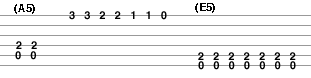
\includegraphics{partfive/shuffleintrotab.png}

\subsection{The Outro}
This is a basic guitar part that will wrap up the song, the last time you play it. It's not very long, and shouldn't be too tough to learn. 

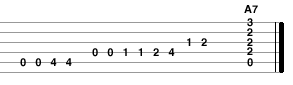
\includegraphics{partfive/shuffleoutrotab.png}

\subsection{The 12 Bar Blues}
This is the main part of the song. The song starts with a simple intro (not shown below), then continues for 12 bars, then repeats (without repeating the intro). The last time the song is played, the last two bars are replaced by the outro. 

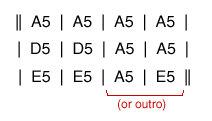
\includegraphics{partfive/shufflebluesform.png}

The above gives the general breakdown of the twelve bar blues, and you'll need to memorize it. Chances are, though, when you hear it played, it will sound logical, and shouldn't be at all hard to memorize.
Although the above diagram shows us generally which chords we will play in each bar, we are going to play something a little more complex than just A5 for four bars, D5 for two bars, etc. To see exactly what you'll play for each bar, study the following: 

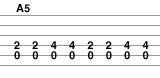
\includegraphics{partfive/shufflea5tab.png}

For each bar of A5, you'll play the above tablature. Play the note on the second fret with your first finger, and the note on the fourth fret with your third finger. 

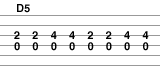
\includegraphics{partfive/shuffled5tab.png}

For each bar of D5, you'll play the above tablature. Play the note on the second fret with your first finger, and the note on the fourth fret with your third finger. 

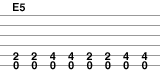
\includegraphics{partfive/shufflee5tab.png}

For each bar of E5, you'll play the above tablature. Play the note on the second fret with your first finger, and the note on the fourth fret with your third finger.

If you listen to the recording, you'll notice there's one small variation not included so far. It is this: the first time through the 12 bar blues, on the 12th bar, we play a different pattern on the E5 chord. This is often done at the end of each 12 bars, because it gives the listener and the band a solid way of knowing that we're at the end of the song form, and we're going back to the beginning again. Here is how you play this very simple pattern: 

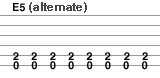
\includegraphics{partfive/shufflee5alternate.png}

And, that's it! Looking at all the above instructions, you're probably going to feel overwhelmed. Pick up your guitar, and try playing through it all... it's actually quite simple, and rather easy to memorize. 

\subsection{Things to try}
\begin{itemize}
\item Loop the 12 bar blues without an intro, and without the outro. Keep repeating the 12 bar form, until you've memorized it.
\item Try playing the intro and outro, along with the song, WITHOUT losing the timing.
\item Play along to the recorded examples.
\item Try playing an A blues scale over the recorded example. This is something we're going to examine further in the future.
\item Be sure you're not hitting open strings that you shouldn't be playing. 
\end{itemize}

\section{The B Minor Chord}
Here's where we take the next big step in our progress as a guitarist... learning about a shape of chord referred to as a "barre chord". The technique of playing barre chords is one which we have utilized when playing the F major chord - using one finger to hold down more than one note.

\subsection{The B minor shape}
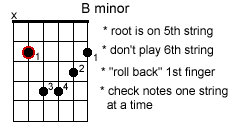
\includegraphics{partfive/bminor.png}

We're going to put your first finger to work on this chord. Your first finger has the job of covering the second fret, from the fifth to first strings (we don't play the sixth string). Next, put your third finger on the fourth fret of the fourth string. Then, add your fourth pinky finger to the fourth fret of the third string. Lastly, place your second finger on the third fret of the second string. Got it? Now, strum the chord, and try not to get upset when most of the notes don't ring clearly.

This is a tough chord at first, no doubt about it! You're going to have to have patience, it WILL sound good soon, but it's going to take some work. Here are some tips that will help you:
\begin{itemize}
\item Very slightly bend your first finger. A straight and rigid finger is not what we're looking for.
\item Roll the finger back slightly, so that more of the side of the index finger closest to the thumb is in contact with the strings.
\item Try slightly pulling the body of the guitar towards your body, using the arm of your picking hand. Also gently pull the neck towards you with your fretting hand. This makes fretting barre chords somewhat easier. 
\end{itemize}

\subsection{Movable chord}
One of the greatest things about the B minor chord shape is that it is a "movable chord". This means that, unlike the chords we've learned so far, we can slide the same shape around to different frets to create different minor chords. The note we're interested in is the note on the fifth string. Whatever note your finger is playing on the fifth string is the type of minor chord it is. If you were to slide the chord up the neck, so that your first finger was at the fifth fret, you'd be playing a D minor chord, since the note on the fifth fret of the fifth string is D. THIS is why learning the note names on the sixth and fifth strings are so important. We'll be getting into different movable chords in the next lesson. 

\subsection{Things to try}
\begin{itemize}
\item Hold the shape of the B minor chord, and play strings one at a time. Correct any notes that aren't ringing clearly.
\item Try moving from other chords to a B minor chord, then back to other chords. This will be a slow and difficult process at first. Keep trying!
\item Try playing different minor chords by moving the B minor shape around to different frets (eg. try playing C\# minor, F minor, G minor, Bb minor, etc.)
\item Do NOT play the sixth string when playing a B minor chord. Pay careful attention to this. 
\end{itemize}

\section{Scale Review}
The blues scale plays a big part in rock in pop music, both in the solos of guitarists, and often within the songs themselves. In lesson three, we learned the basics of the blues scale. Now, we'll review the scale, and explore it a little bit further. 

\subsection{The Blues Scale}
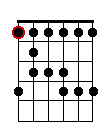
\includegraphics{partfive/bluesscale2.png}

If you're having trouble remembering exactly how to play the blues scale, have a look at the diagram on the left. Truthfully, it's one of the easier scales you'll learn.. probably because your first finger starts on the same fret of each string. Play the scale forwards and backwards several times.

What fret you start this scale at depends on which scale you'd like to play.. like the B minor chord we learned in this lesson, the blues scale is "movable". What type of blues scale you're playing depends on which fret you start at. If you start the scale with your first finger on the fifth fret of the sixth string (the note A), you're playing an "A blues scale". If you start the scale with your first finger on the eighth fret of the sixth string, you're playing a "C blues scale". 

\subsection{Uses of Blues Scale}
If you're interested in learning to play guitar solos, you'll want to spend a whole lot of time with the blues scale. Many pop, rock, and blues guitarists use the blues scale almost exclusively in their solos. The basic premise is this: a guitarist will play a series of notes from the blues scale, which sound good together. Learning to do this well takes experimentation and practice, but it gets easier.

Many songwriters use parts of the blues scale as the foundation for their songs. Led Zeppelin did this often: in the song Heartbreaker for example, the blues scale is used extensively in the main "guitar riff". Eric Clapton used the blues scale too, for the riff in Cream's Sunshine of Your Love. 

\subsection{Things to try}
\begin{itemize}
\item Play the scale forwards and backwards. Try starting in the middle of the scale, and finishing it, going forwards, and backwards. In short... memorize it well!
\item Experiment with playing various notes from the A blues scale along with this week's blues shuffle (click to hear audio)
\item If you have an interest in learning more about soloing, study the older archived lesson Learning to Improvise.
\item Play around with the notes in the blues scale, and see if you can't come up with a cool "guitar riff" that could be the basis of a song. 
\end{itemize}

\section{Learning Songs}
Since we've now covered all the basic open chords, plus power chords, and now the B minor chord, there are a countless number of songs to tackle. This week's songs will be focus on both open and power chords. 

Like a Rolling Stone - performed by Bob Dylan
NOTES: Try strumming this one as Down, Down, Down, Down up. Some rather quick chord changes in this song will keep you on your toes!
Wonderful Tonight - performed by Eric Clapton
NOTES: Here's a nice easy one. Strum chords 8x downwards each, with a few exceptions (use your ears to tell you which ones).Instead of D/F\#, play Dmajor. If you're brave, you can try the lead guitar part (it's not that hard).
Hotel California - performed by The Eagles
NOTES: okay this one is tough... since it uses a Bminor, and many other chords. There is also a new chord: F\#, which you'll play like this: play an Fmajor chord, and slide your fingers up one fret (so your first finger is barring the first and second strings, second fret).. only play strings four through one for this chord. When you see Bm7, play Bminor. Good luck!
Otherside - performed by The Red Hot Chili Peppers
NOTES: This song is surprisingly easy. Learn the opening single note riff, and the chords (don't worry about the notes below the chords for now). Strum chords: down, down up, up down up. 

\section{Practice Schedule}
Realistically, in order to play the B minor chord properly, you're going to have to invest some time in practicing. Here is a routine I would suggest, in order to keep your progress moving smoothly.
\begin{itemize}
\item Make sure your guitar is in tune (review how to tune).
\item Warm up by playing the blues scale, forwards and backwards, several times. Play slowly, use alternate picking, and make sure each note rings clearly.
\item Play through all chords you know, including the open chords, power chords, and the B minor chord. Be sure you know the name and shape for each chord.
\item Spend time reviewing the note names on the sixth and fifth string. Memorizing these notes is essential. Start by memorizing a few notes on each string.
\item Review all strumming patterns we've covered. We've learned patterns in lesson two, lesson three, and lesson four. Try switching from chord to chord while using these patterns.
\item Review the F major chord. It might not sound perfect yet, but chances are, if you've been practicing it, it's getting better and better. Keep it up.
\item Try to play all of the songs above. Don't get frustrated if a song is too tough for you. Take a deep breath, and try some more. If you're feeling overwhelmed, move to an easier song, or try songs from previous lessons. 
\end{itemize}
As we continue to learn more and more material, it becomes easy to overlook the techniques we learned during earlier lessons. They are all still important, so it is advisable to keep going over older lessons, and be sure you're not forgetting anything. There is a strong human tendency to only practice things which we are already quite good at. You'll need to overcome this, and force yourself to practice the things you are weakest at doing.

If you're feeling confident with everything we've learned so far, I suggest trying to find a few songs you're interested in, and learn them on your own. You can use the guitar tab area of the site to hunt down the music that you'd enjoy learning the most. Try memorizing some of these songs, rather than always looking at the music to play them.

In lesson six, we'll learn more strumming patterns, a few 7th chords, another barre chord, new songs, and much more. Have fun until then, and keep practicing! 


  \chapter{Lesson 6}
\section{Overview}
In lesson one of this special feature on learning the guitar, we were introduced to the parts of the guitar, learned to tune the instrument, learned a chromatic scale, and learned Gmajor, Cmajor, and Dmajor chords. Guitar lesson two taught us to play Eminor, Aminor, and Dminor chords, an E phrygian scale, a few basic strumming patterns, and the names of the open strings. In guitar lesson three, we learned how to play a blues scale, Emajor, Amajor, and Fmajor chords, and a new strumming pattern. Lesson four introduced us to power chords, basic note names on the sixth and fifth string, and new strumming patterns. Most recently, in lesson five, we studied sharps and flats, were introduced to barre chords, learned to read tab, and learned a basic 12 bar blues. If you are not familiar with any of these concepts, it is advised that you revisit these lessons before proceeding.

\subsection{What You'll Learn in Lesson Six}
Hopefully, you won't find this lesson so tough. We'll tackle a few new chords, which are called 7th chords. Also, we'll learn a few more of the tricky barre chords. Plus, a new handy strumming pattern. Additionally, if you looking for warm-up exercises, we'll learn a movable chromatic scale pattern. And, as usual, we'll get down to applying what we've learned, by using these techniques in various songs. 

Are you ready? Good, let's start guitar lesson six.

\section{Chromatic Scale}
If you think all the way back to lesson one, you'll recall we previously learned a chromatic scale pattern. We used that scale as a means of getting our fingers accustomed to pressing down frets on the guitar. Here again, we will study another method of playing this scale, except farther up on the neck. The goal of learning this new scale position is to get our fretting hand to move smoothly and quickly all over the neck.

Before we begin, let's clarify exactly what a "chromatic scale" is. In Western music, there are 12 different musical pitches (A, Bb, B, C, Db, D, Eb, E, F, Gb, G, Ab). The chromatic scale includes EACH of these 12 pitches. So, we could actually play a chromatic scale simply by sliding our finger up one string, playing each fret.

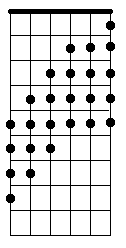
\includegraphics{partsix/chromaticscale2octave.png}

Our reason for learning the chromatic scale, at this point, is simply as a means of improving our finger technique. Start by placing your first finger on the fifth fret of the sixth string, and play that note with a downstroke. Follow that by using your second finger to play the sixth fret of the sixth string (with an upstroke). Then, your third finger should play the seventh fret on the sixth string, and lastly, your fourth (pinky) finger should play the eighth fret.

Now, move on to the fifth string. Playing this string will require a "position shift" in your fretting hand. Move your hand position down one fret, starting on the fourth fret of the fifth string with your first finger. Play each note on that string, as you did on the sixth. Repeat this process on each of the sixth strings (notice that you DON'T switch positions on the second string. This is because the second string is tuned differently than the other five.)

When you reach the first string, play the first fret with your first finger, as usual. Then, immediately switch positions, and also play the second fret with your first finger. This step allows you to reach the fifth fret, thus completing the two octave A chromatic scale. When you've reached the end of the scale, try playing it backwards.

\subsection{Remember}
\begin{itemize}
\item Keep your fretting hand as loose as possible. Don't grip the neck too tightly, or switching positions will become more difficult.
\item Try and set up a steady rhythm while playing the scale. Focus on making it sound as fluid as possible. Play the scale as slowly as necessary in order to make the tempo even throughout.
\item Alternate picking here is extremely important. Don't allow yourself to be careless.
\item Try looking at your picking hand while you play, instead of at your fretting hand. Is it doing everything as efficiently as it should?
\item Don't rush through this exercise, and don't allow yourself to get frustrated. Pay careful attention to any minor flaws in your technique, and try to remedy them.
\end{itemize}
Let's move on to learning the 7th chords... 

\section{Open 7th Chords}
Up until this point, we've dealt with only major, minor, and 5th(power) chords. While these are all extremely common, there are many other types of chords, each of which have their own unique sound. The 7th chord (aka the 7 chord) is one of these many different chords. This week, we'll look at a few of these 7th chords, in open position (not barre chords).

\subsection{Playing a G7 chord}
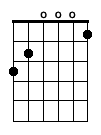
\includegraphics{partsix/openg7.png}

Start playing the G7 chord by placing your third finger on the third fret of the sixth string. Next, put your second finger on the second fret of the fifth string. Lastly, place your first finger on the first fret of the first string. Make sure your fingers are nicely curled, and give the chord a strum. Voila! Notice that this G7 chord looks quite similar to a Gmajor chord - only one note is different.

\subsection{Playing a C7 chord}
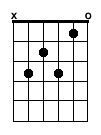
\includegraphics{partsix/openc7.png}

The C7 chord shouldn't give you too much trouble - it again is very close in formation to a Cmajor chord, with only one note being different. Play this chord as follows - form a Cmajor chord, by placing your third finger on the third fret of the fifth string, your second finger on the second fret of the fourth string, and your first finger on the first fret of the second string. Now, place your fourth (pinky) finger on the third fret of the third string. Strum the bottom five strings, and you're playing a C7 chord.

\subsection{Playing a D7 chord}
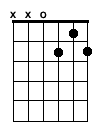
\includegraphics{partsix/opend7.png}

As with the previous two chords, you'll notice the D7 chord is rather similar to the Dmajor chord. Start by placing your second finger on the second fret of the third string. Next, place your first finger on the first fret of the second string. Lastly, put your third finger on the second fret of the first string. Strum the bottom four strings, and you're playing a D7 chord.

\subsection{Remember}
\begin{itemize}
\item In all cases, you should be checking each chord for accuracy by playing strings one at a time. If each string does not ring clearly, find out why not, and correct the problem.
\item Be sure you're not strumming strings with an "x" above them in the diagrams. Playing these strings will almost always result in chords sounding yucky.
\item Practice moving from chord to chord, saying each one aloud as you're playing it. It is very important to memorize the chord name as well as the chord shape.
\end{itemize}
Let's move on to learning more barre chords.

\section{Barre Chord Basics}
In lesson five, we took the big step of beginning to play barre chords, by learning a B minor chord. If you haven't practiced B minor recently, I'd suggest taking some time to try and master it before continuing. Knowing the note names on the sixth and fifth strings is also required to properly use barre chords.

The barre chords in lesson six will be somewhat similar to the shape we learned previously. These chords are difficult to play at first, but with practice, they will begin to open up whole new worlds in your guitar playing. 

\subsection{The F major barre shape}
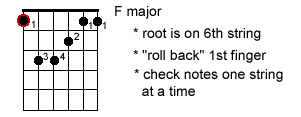
\includegraphics{partsix/fmajorbarre.png}

As with the Bminor chord, the key to playing this F major shape well is getting your first finger to flatten across the entire fretboard. Try rolling your first finger back slightly, towards the headstock of the guitar. Once your first finger feels firmly in place, try adding your other fingers to complete the chord. Playing this shape well requires much practice, but it WILL get easier, and soon you won't understand why these shapes ever caused you any problems.

As with the Bminor chord in our last lesson, this major chord shape is a "movable chord". Meaning, we can slide this chord up and down the neck, in order to play different major chords. The root of the chord is on the sixth string, so whatever note you are holding down on the sixth string is the letter name of that major chord. For example, if you were playing the chord at the fifth fret, it would be an A major chord. If you were playing the chord at the second fret, it would be a Gb major chord (aka F\# major). 

\subsection{The F minor barre shape}
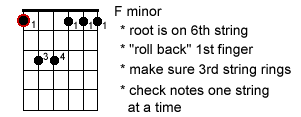
\includegraphics{partsix/fminorbarre.png}

This chord is very similar to the Fmajor shape above. There is only one slight difference... your second finger is not used at all. Your first finger is now responsible for fretting four of the six notes in the chord. Although it looks slightly easier to play than the major chord, many guitarists initially have a harder time making the chord sound correct. When playing the chord, pay careful attention to the third string. Is the note ringing clearly? If not, try and correct the problem. Playing these chords well will take time - don't allow yourself to get frustrated! It took me months to get them to sound as clearly as I liked. Try to keep that in mind.

Again, this minor chord is a movable shape. If you played this chord on the 8th fret, you'd be playing a C minor chord. On the 4th fret, you'd be playing an Ab minor chord (aka G\# minor). 

\subsection{Using Barre Chords}
Once you get the hang of playing these new shapes, you can start to use them everywhere. One of the best ways to practice barre chords is to try using them in songs you already know how to play. Simply use barre chords instead of the open chords you were using previously. Try playing Leaving on a Jet Plane using the major barre chord shapes, for example. 

\subsection{Things to Try}
\begin{itemize}
\item If you're feeling overwhelmed, try playing any songs you know that use an F major chord. Play all other chords in the song with "regular" open chord shapes, but try the barre shape for the F major.
\item Make a sincere effort to learn note names on the sixth and fifth string. I can't stress enough how important this is to learn.
\item Play barre chords for just a few minutes every day - but play them EVERY DAY. You'll be surprised how quickly you learn them. 
\end{itemize}
Now, let's move on to a new strumming pattern. 

\section{Strumming Patterns}
In lesson two, we learned all about the basics of strumming the guitar. We added another new strum to our repetoire in lesson three. In lesson four, we studied yet another common strumming pattern. If you still aren't comfortable with the concept and execution of basic guitar strumming, it is advised that you return to those lessons and review. 

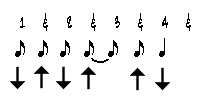
\includegraphics{partsix/strum5.png}

If you didn't have any problems with prior strumming patterns, then this one won't give much difficulty either. This is another common strum, which is just a slight variation of several strums covered earlier.

Let's take a moment to listen to what this strumming pattern sounds like at a slow tempo. Try and internalize the rhythm of this strum before you even attempt to play it on guitar. Say "down up down up up down" along with the audio clip. Once you feel comfortable that you know the rhythm properly, pick up your guitar, hold down a G major chord, and try strumming along.

If you can't seem to get it right, spend more time practicing the rhythm away from your guitar. I can't stress this enough - the key to learning strumming patterns is to be able to "hear" the pattern in your head before you try and play it. Once you've gotten the hang of it, you'll want to try playing the same pattern at a faster tempo 

\subsection{Remember}
\begin{itemize}
\item If you are playing an acoustic guitar, make sure to strum directly over the sound hole
\item On electric guitar, strum over the body (different locations will give you different sounds), not over the neck
\item Make sure all strings are ringing clearly
\item Make sure the volume of your downstrums and upstrums are equal
\item Be careful not to strum too hard, as this often causes strings to rattle, and produces an undesirable sound
\item Be careful not to strum too softly, as this will produce a "wimpy" sound. Your pick should be striking the strings with a relatively firm, even stroke
\item Think of your elbow as being the top of a pendulum; your arm should swing up and down from it in a steady motion, never pausing at any time.
\item Having said that, the bulk of the picking motion should come from a rotation of the wrist, rather than from the forearm. Be sure not to keep your wrist stiff when playing. 
\end{itemize}
Let's use these new chords and strumming patterns by learning some new songs. 

\section{Learning Songs}
Since we've now covered all the basic open chords, plus power chords, and now the B minor chord, there are a countless number of songs to tackle. This week's songs will be focus on both open and power chords. 

Best of my Love - performed by The Eagles
NOTES: We can use our newest strum to play this song, which also includes a G7 chord we learned this week. The bridge includes an Fminor barre chord, but if you can't play that yet, at least attempt the verse.
Californication - performed by The Red Hot Chili Peppers
NOTES: This is the title track from the band's 2000 album. Some single notes to learn, but the song isn't too hard.
Hotel California - performed by The Eagles
NOTES: we did this one last lesson as well, but you'll be better equipped to play it now. Try using full barre chords for Bminor and F\#major. When you see Bm7, play Bminor. Strum: down down up up down up
Yer So Bad - performed by Tom Petty
NOTES: if you're getting frustrated, here's a nice, easy song to learn. Just a few chords, none of them new. For now, we'll strum it down down up up down up.

\section{Practice Schedule}
Don't spend all of your time trying to play barre chords - chances are you'll just end up frustrated with very sore fingers. If you want to conquer them, however, you'll have to put in a few minutes worth of work every time you pick up your guitar. Here are some other things you'll want to practice after this lesson:
\begin{itemize}
\item First, make sure your guitar is in tune).
\item Warm up by playing the new chromatic scale slowly and accurately. Try not to hesitate when switching strings.
\item Review the new 7th chords, plus open chords, power chords, the B minor barre chord, and this week's barre chords. We've learned a lot, so it's important to keep them all organized in your mind.
\item Review all strumming patterns we've covered. We've learned patterns in lesson two, lesson three, lesson four, and lesson six. Try switching from chord to chord while using these patterns.
\item Try to play all of the songs above, plus keep playing those from previous lessons. Try committing one or several songs to memory. Pick an easy one to start with. 
\end{itemize}
As we continue to learn more and more material, it becomes easy to overlook the techniques we learned during earlier lessons. They are all still important, so it is advisable to keep going over older lessons, and be sure you're not forgetting anything. There is a strong human tendency to only practice things which we are already quite good at. You'll need to overcome this, and force yourself to practice the things you are weakest at doing.

If you're feeling confident with everything we've learned so far, I suggest trying to find a few songs you're interested in, and learn them on your own. You can use the easy guitar tab area of the site to hunt down the music that you'd enjoy learning the most. Try memorizing some of these songs, rather than always looking at the music to play them.

In lesson seven, we'll another barre chord (our last for a little while), hammer-on and pull-off techniques, new songs, and much more. Be sure you're always having fun while you're playing, and keep smiling! 


  \chapter{Appendix}
\section{Leaving on a Jet Plane} \label{sec:song1}
Words and Music by John Denver
\begin{verbatim}
       G     /     /     /   C    /   /   /
All my bags are packed, I'm ready to go
    G    /    /    /  C    /    /   /
I'm standing here outside your door
  G     /   /   /  C  /   /   /  D  ///////
I hate to wake you up to say goodbye
        G     /   /       /    C  /   /   /
But the dawn is breakin' it's early morn
     G  /   /      /    C        /   /   /
The taxi's waitin' he's blowin' his horn
  G  /   /   /  C  /    /   /   D  ///////
Already I'm so lonesome I could die


Chorus:
   G  /  /   /  C    /   /  /  
So kiss me and smile for me 
G    /   /    /     C    /   /   /
Tell me that you'll wait for me
G    /   /    /     C  /   /   /  D ///////
Hold me like you'll never let me go
           G / / /  C  /  /   /  
'Cause I'm leavin' on a jet plane
G  /    /     /  C    /    /    /  
 Don't know when I'll be back again
G  /  /  /  C    /   /   /  D ///////
        Oh, babe, I hate to go....

Verse 2:
There's so many times I've let you down
So many times I've played around
I tell you now, they don't mean a thing
Every place I go, I'll think of you
Every song I sing, I'll sing for you
When I come back I'll bring your wedding ring

CHORUS

Verse 3:
Now the time has come to leave you
One more time, let me kiss you
Then close your eyes, I'll be on my way
Dream about the days to come
When I won't have to leave alone
About the times I won't have to say

CHORUS

end on G chord
\end{verbatim}

\section{The Gambler} \label{sec:song2}
words and music by Kenny Rogers
\begin{verbatim}
     G                          C               G
On a warm summer's evenin' on a train bound for nowhere,
  C               G                C                 D
I met up with the gambler; we were both too tired to sleep.
   G                               C             G
So we took turns a starin' out the window at the darkness
     C           G        D               G
'til boredom overtook us, and he began to speak.

         G                             C                G
He said, "Son, I've made a life out of readin' people's faces,
    C                  G                 C                   D
and knowin' what their cards were by the way they held their eyes.
       G                               C                 G
And if you don't mind my sayin', I can see you're out of aces.
      C             G            D             G
For a taste of your whiskey I'll give you some advice."

     G                           C                  G
So I handed him my bottle and he drank down my last swallow. 
C                G             C              D
Then he bummed a cigarette and asked me for a light.
        G                                C                 G
And the night got deathly quiet, and his face lost all expression.
                 C                    G             D                G
Said, "If you're gonna play the game, boy, ya gotta learn to play it right.

CHORUS:
           G                     C             G
You got to know when to hold 'em, know when to fold 'em,
C            G         C                D
know when to walk away and know when to run.
          G                            C              G
You never count your money when you're sittin' at the table.
                 C          G        D                 G
There'll be time enough for countin' when the dealin's done.


D                            C             G
Ev'ry gambler knows that the secret to survivin'
   C              G           C                   D
is knowin' what to throw away and knowing what to keep.
       G                         C              G
'Cause ev'ry hand's a winner and ev'ry hand's a loser,
        C                 G              D           G
and the best that you can hope for is to die in your sleep."

    G                               C                       G
And when he'd finished speakin', he turned back towards the window,
C               G             C            D
crushed out his cigarette and faded off to sleep.
    G                             C                 G
And somewhere in the darkness the gambler, he broke even.
    C            G                D                G
But in his final words I found an ace that I could keep.

CHORUS 2x and end...
\end{verbatim}

\section{Brown Eyed Girl} \label{sec:song3}
Words and music by Van Morrison
\begin{verbatim}
   G               C       G             D  
Hey, where did we go   days when the rain came
Whatever      happened to Tuesday and so slow

G              C         G               D     
Down in  the   hollow    playing    a   new game 
Going down the old mine with a transistor radio

G               C                 G              D         
Laughing and a running, hey hey   Skipping and a jumping
Standing in the sunlight laughing hiding 'hind a rainbow's wall

G              C            G           D
in the misty   morning fog, ah   with   our hearts a thumpin'
Slipping and a sliding     all along the waterfall

    C     D             G      Em
and you,  my brown eyed girl 
and you,  my brown eyed girl 

C      D           G     D
You, my brown eyed girl
You, my brown eyed girl
  
BRIDGE:
 
D
Do you remember when we used to sing
 
G         C           G              D
Sha la la la la la la la la la la te da  Just like that
 
G         C           G              D         G
Sha la la la la la la la la la la te da  la te da
 
VERSE 3:
So hard to find my way 
Now that I'm all on my own
I saw you just the other day
My, how you have grown
Cast my memory back there Lord
Sometimes I'm overcome thinkin' 'bout it
Makin' love in the green grass
Behind the stadium
With you, my brown eyed girl
You, my brown eyed girl
 
REPEAT BRIDGE AND END
\end{verbatim}

\section{Take It Easy} \label{sec:song4}
The Eagles
\begin{verbatim}
           G                         
Well I'm a runnin' down the road try'n to loosen my load
                     D     C
I've got seven women on my mind
G                       D
Four that wanna own me, two that wanna stone me
C                              G
One says she's a friend of mine
         Em            C G
Take it easy, take it easy
              Am                C                 Em
Don't let the sound of your own wheels drive you crazy
          C                G
Lighten up while you still can
           C                G
Don't even try to understand
            Am                 C                     G
Just find a place to make your stand,  and take it easy


            G
Well, I'm a standin' on a corner in Winslow, Arizona
            D        C
Such a fine sight to see
       G                 D
It's a girl my lord in a flat-bed Ford
        C                        G
Slowin' down to take a look at me
          Em              C G
Come on, baby, don't say maybe
        Am                 C                 Em
I gotta know if your sweet love is gonna save me
       C               G                  C             G
We may lose and we may win, though we may never be here again
        Am              C                G
So open up I'm climbin' in, so take it easy


            G
Well, I'm a runnin' down the road tryin' to loosen my load
                       D     C
Got a world of trouble on my mind
G                       D                          C              G
Lookin' for a lover who won't blow my cover, she's so hard to find
         Em             C G
Take it easy,  take it easy
              Am                C                 Em
Don't let the sound of your own wheels make you crazy
        C G             C  G
Come on baby, don't say maybe
        Am                 C             G           C   Em   
I gotta know of your sweet love is gonna save me


-----------------------------------------------------------
Chords used:

        E A D G B e
       +-----------+
Am      x 0 2 2 1 0
C       0 3 2 0 1 0
D       x 0 0 2 3 2
Em      0 2 2 0 0 0
G       3 x 0 0 0 3
       +-----------+
\end{verbatim}

\section{Mr Tambourine Man} \label{sec:song5}
The Byrds
\begin{verbatim}
Intro:
D   G   A

Chorus:
G           A               D               G
Hey! Mister Tambourine Man, play a song for me.
        D                G     Em        A
I'm not sleepy and there is no place I'm going to.
G           A               D               G
Hey! Mister Tambourine Man, play a song for me.
       D             G       Em        A         D   G   D
In the jingle jangle morning I'll come following you.

         G                  A          D                 G
Though I know that evenin's empire has returned into the sand.
D                G             D               G
Vanished from my hand, left me blindly here to stand 
    Em        A
but still not sleeping!
   G          A             D             G      D              G
My weariness amazes me, I'm branded on my feet I have no one to meet.
        D             G            Em       A
And the ancient empty street's too dead for dreaming.

Chorus

Take me on a trip upon your magic swirlin' ship
My senses have been stripped, my hands can't feel the grip, 
my toes too numb to step, wait only for my boot heels
to be wandering
I'm ready to go anywhere, I'm ready for to fade
Into my onw parade cast your dancing spell my way,
I promise to go under it

Chorus

Though you might hear laughin' spinnin' swingin' madly across the sun
It's not aimed at anyone, it's just escapin' on the run
And but for the sky there are no fences facin'
And if you hear vague traces of skippin' reels of rhyme
To your tambourine in time, it's just a ragged clown behind
I wouldn't pay it any mind, it's just a shadow you're
seein' that he's chasing

Chorus

Then take me dissapearin' through the smoke rings of my mind
Down the foggy ruins of time, far past the frozen leaves
The haunted, frightended trees out to the windy beach
Far from the twisted reach of crazy sorrow
Yes, to dance beneath the diamond sky with one hand wavin' free
Silhouetted by the sea, circled by the circus sands
With all memory and fate drive deep beneath the waves
Let me forget about today until tomorrow
\end{verbatim}

\end{document}
